\subsection{Einleitung}
Der signifikanteste Unterschied zwischen üblichen Dateisynchronisationsdiensten
und \sblit besteht im Verzicht eines Servers. Anders als im Kapitel 1.1.2. erklärt,
findet die Kommunikation zwischen zwei Endgeräten nicht über einen Server statt,
sondern über eine direkte verschlüsselte Verbindung zwischen diesen zwei Geräten.

Durch diesen Ansatz, fällt die zentrale Sammelstelle von Nutzerdaten
weg und dem Datendiebstahl von Hackern wird ein Riegel vorgeschoben. Außerdem
wird kein betreibendes Unternehmen mehr benötigt, um Server zu warten, womit auch
die einheitliche Anlaufstelle für staatliche Sicherheitsbehörden und Geheimdienste
nicht mehr existiert.

\subsection{Herausforderungen}
Mit dem Weglassen eines Servers, entstehen aber auch viele Herausforderungen,
wenn der volle Funktionsumfang eines üblichen Dateisynchronisationsdienstes
trotzdem gewährleistet werden soll.

So fehlt der öffentliche Server als bekannter \glqq{} Mittelmann \grqq{} in der Kommunikation
zwischen den Clients, sodass sich diese über das Internet hinwegüber mit einem
eigenen Protokoll finden, um eine direkte Verbindung erfolgreich aufbauen zu können.
Mehr zu den genauen Herausforderungen beim Verbindungsaufbau und
die Bewältigung dieser folgt im Kapitel ...
%TODO Kapitel eintragen mit verlinken.
Der Server dient aber nicht aber nicht nur als \glqq{} Mittelmann \grqq{} damit die Clients
miteinander kommunizieren können. Er dient nämlich auch als \gls{filecloud},
also als Zwischenspeicher für Daten. Dieser ist nämlich essenziell, wenn man
Dateien ohne große Komplikationen synchronisieren will. Um zu erklären warum das
so ist, gehen wir von folgendem Szenario bei Verwendung eines Servers aus:
%TODO Bild einfügen, auf dem bei Dropbox ein Client nicht erreichbar ist.
Der Rechner in der Schule ist eingeschaltet, das Gerät zu Hause nicht. Wird nun
eine bereits synchronisierte Datei auf dem Schulrechner bearbeitet, wird eine Kopie dieser wie
üblich auf die \gls{filecloud}, also den Server hochgeladen. Wenn die Schule vorbei ist,
wird der Schulrechner abgedreht und zu Hause kann die neuste Version der geänderten Datei beim
Einschalten des Heim-PCs trotzdem übertragen werden, da diese in der \gls{filecloud}
zwischengespeichert wurde und sie von dort aus gesendet wurde.

Ohne den Server als \gls{filecloud}, wäre die alte Version der Datei bearbeitet worden, sodass zwei
neue Versionen der Datei existieren würden. Dies nennt man einen \gls{versionconflict}.

Mit dem Verzicht auf den Server, muss also eine alternative \gls{filecloud} benutzt
werden, um Dateien zwischenspeichern zu können, sodass in vorherigen Szenario ohne Server
keine \glspl{versionconflict} auftreten.

Deshalb kommt bei \sblit eine dezentrale \gls{filecloud} zum Einsatz. Anstelle
eines zentralen Speicherns durch einen Server, wird auf den Speicherplatz der
verschiedenen Nutzern von \sblit zurückgegriffen. Diese dezentrale \gls{filecloud}
besteht also aus den verteilten Speicherplätzen verschiedenster Nutzer.

Dieses Prinzip funktioniert durch ein faires Abkommen zwischen den \sblit-Nutzern,
sogenannten \glspl{partnership}. Grundsätzlich sind \glspl{partnership} einfach eine
Vereinbarung mit anderen, teilweise sogar fremden Nutzern, sich gegenseitig Speicherplatz
freizugeben. Eine \gls{partnership} wird entweder automatisch mit unbekannten Nutzern
geschlossen, oder durch den Nutzer selbst mit Bekannten. Genauer wird auf dieses Thema allerdings weiter hinten im Buch im
Kapitel ... eingegangen.
%TODO Kapitel eintragen mit verlinken des selbigen
Die Dateien werden aber natülich nicht nach einer verschlüsselten Übertragung unverschlüsselt
auf den teilweise fremden \glspl{partnerdevice} gespeichert. Verschlüsseln ist dabei
natürlich Pflicht, es wurde allerdings noch einen Schritt weiter gedacht. Generell
hat bei \sblit nämlich nur der Nutzer, dem der die Datei auf den Partnergeräten speichert und
dessen \glspl{syncpartner} Zugriff auf die vollständigen Dateien.

Wenn also ein oder mehrere \glspl{syncpartner} nicht erreichbar sind.

Bei \sblit werden Dateien anstatt über einen Server, nämlich über verschlüsselte
Verbindungen zwischen zwei Endgeräten direkt übertragen.
Oft kommt es allerdings vor, dass \glspl{syncpartner} beim Verändern von
Dateien nicht erreichbar sind und keine Verbindung aufgebaut und auch
keine Datei synchronisiert werden kann.
Mit dem Senden einer neuen Version von Dateien zu warten,
bis beide Clients gleichzeitig erreichbar sind, hätte eine zu große Zeitspanne
zur Folge, in der viele Versionskonflikte auftreten könnten.
Deshalb verwendet \sblit eine Cloud, um Dateien für nicht erreichbare
Synchronisationspartner extern zwischenspeichern zu können. Die Cloud bildet
sich dabei aber nicht aus einem Server, wie üblich, sondern aus einem \gls{p2pnet}
aller Nutzer von \sblit. Diese dezentrale \gls{filecloud} wird
mit sogenannten \glspl{partnership} realisiert. Dabei geht es darum, dass sich
User, die sich gegenseitig nicht kennen müssen, einander ihre Daten direkt über
verschlüsselte Kanäle auf den Geräten des jeweiligen anderen speichern.
Um die Dateien nicht nur sicher zu übertragen, sondern auch zwischenzuspeichern,
ohne, dass Dritte Zugriff haben, werden die zu
synchronisierenden Dateien in Blöcke aufgeteilt und verschlüsselt. Diese
verschlüsselten Blöcke werden dann verteilt auf die \glspl{partnerdevice} gespeichert,
sodass diese fremden User nichts damit anfangen können, da sie weder den
Schlüssel zum Entschlüsseln, noch die Informationen über den Ort der restlichen
Blöcke besitzen. Diese befindet sich ausnahmslos nur bei dem User, zu dem die
Blöcke gehören.

\subsection{Szenario}
Bei \sblit wird der Inhalt eines Ordners synchronisert, der bei der
Konfiguration angegebenen wurde. Sobald sich Dateien innerhalb des Ordners
ändern, wird die neue Version der Datei kopiert und die Kopie wird den
erreichbaren Synchronisationspartnern über eine direkte verschlüsselte Verbindung
gesendet.

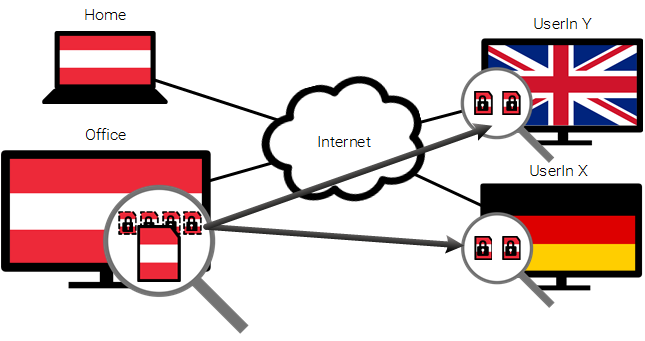
\includegraphics[]{images/sblit_1}
%\caption{Übertragung der Datei zwischen zwei erreichbaren Hosts}.

Für Synchronisationspartner, die nicht erreichbar sind, wird die Datei in der dezentralen
\gls{filecloud} zwischengespeichert. Die Datei wird kopiert und in Blöcke
aufgeteilt. Diese Blöcke werden mit dem privaten Schlüssel des Clients
verschlüsselt und verteilt auf den \glspl{partnerdevice} gespeichert.

Da die Erreichbarkeit der Partnergeräte, auf denen die veschlüsselten
Datei-Blöcke gespeichert sind, nicht gewährleistet ist, wird die Datei mehrmals
in die dezentrale \gls{filecloud} gespeichert, sodass nur ein Bruchteil der
Partnergeräte erreichbar sein muss, um auf die vollständige Datei zugreifen zu
können.

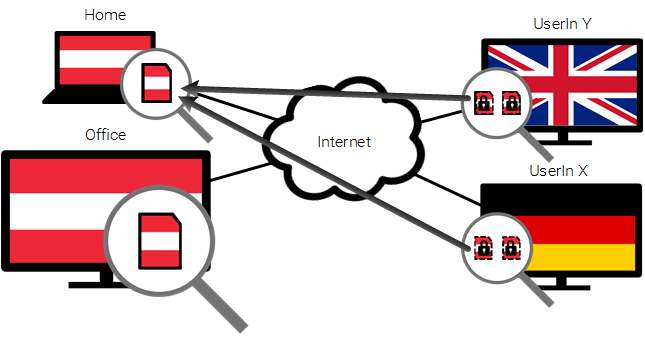
\includegraphics[]{images/sblit_2}
%\caption{Hochladen der Datei in die dezentrale \gls{filecloud}}.

Sobald der \gls{syncpartner}, hier Home wieder hochgefahren ist, fordert er die
verschlüsselten Dateiblöcke von den \glspl{partnerdevice} an. Die Blöcke werden
übertragen, entschlüsselt und zu dervollständigen Datei zusammengesetzt.

Die Datei wurde also über die Partnergeräte synchronisiert, die eine dezentrale
\gls{filecloud} darstellen.

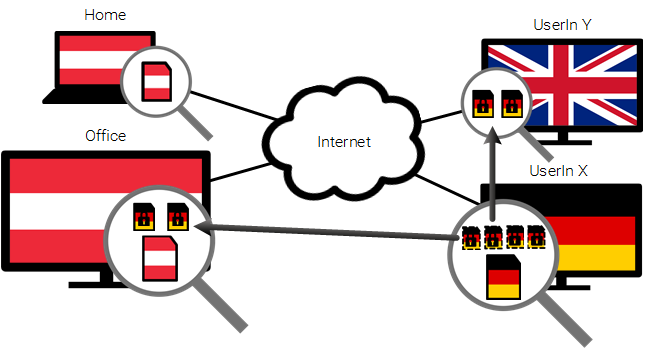
\includegraphics[]{images/sblit_3}
%\caption{Gegenseitiges Speichern von Dateiblöcken (Konzept einer \gls{partnership})}.

Im Gegenzug, dass man Daten auf Geräten anderer speichern darf, gibt man selbst
Speicherplatz für diese User frei, in dem die von ihnen verschlüsselten
Dateiblöcke zwischengespeichert werden können. Der für andere User freigegebene
Speicherplatz beträgt dabei die Speichermenge, die man selbst bei anderen Usern
beansprucht.
